\chapter{Testing Models of Signal Transmission Along Nerve Axons}
\thispagestyle{fancy}
\fancyhead[RE,LO]{Experiment \thechapter}

\begin{wrapfigure}{r}{0.45\textwidth}
  \vspace{-25pt}  
  \begin{center}
  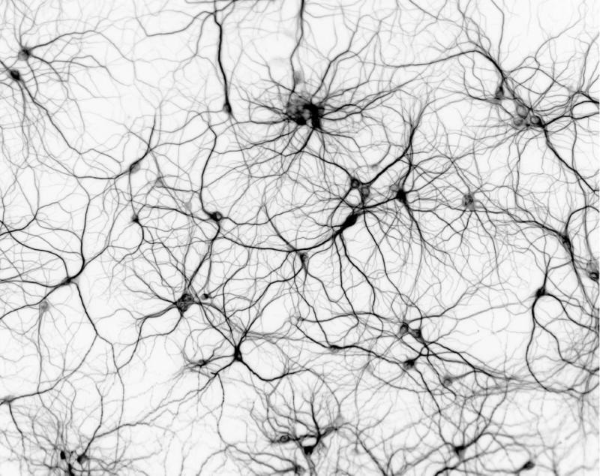
\includegraphics[width=0.43\textwidth]{neural_nets}
  \end{center}
  \caption{Neurons form networks for information flow.}
  \label{fig:neural_net}
  \vspace{-5pt}
\end{wrapfigure}
Nerve impulses travel in our bodies as electrical signals. 
Whether its seeing or hearing something, controlling a muscle, or just thinking, the transmission process along a nerve cell, or neuron, is the same: a sufficient stimulus received by the cell body (\emph{soma}) initiates a change in the potential difference across the membrane, or action potential, which travels along the axon to be transferred through a synapse to the other neurons or muscle cells. 
[See figures~\ref{fig:neural_net} and \ref{fig:neuron}.]
A single axon can be a meter or more long, like those connecting our toes to our spinal cords, so action potentials must travel a long way.
You may have learned in a biology course that for an action potential to be transmitted from one end of an axon to another, it must be regenerated repeatedly along its length.
We call this active transport and it is accomplished by voltage-gated ion channels, as discussed in the appendix to this lab.
Why is active transport necessary?
Couldn't we simply apply a potential difference to the end of a nerve axon and expect that signal to travel along the axon to its final destination, the spinal cord and then the brain?
This alternate type of signal transmission is called passive transport. 
In this two week lab sequence, transport is a feasible method of signal transmission. 
We will also be considering some adaptations to the simple cylinder model of a nerve axon (see below) that can increase the speed of signal transfer – surely a faster response is advantageous to survival in a species!

\subsection*{Simple cylinder model of a nerve axon: structure and properties}
\begin{wrapfigure}{R}{0.45\textwidth}
  \vspace{-25pt}  
  \begin{center}
    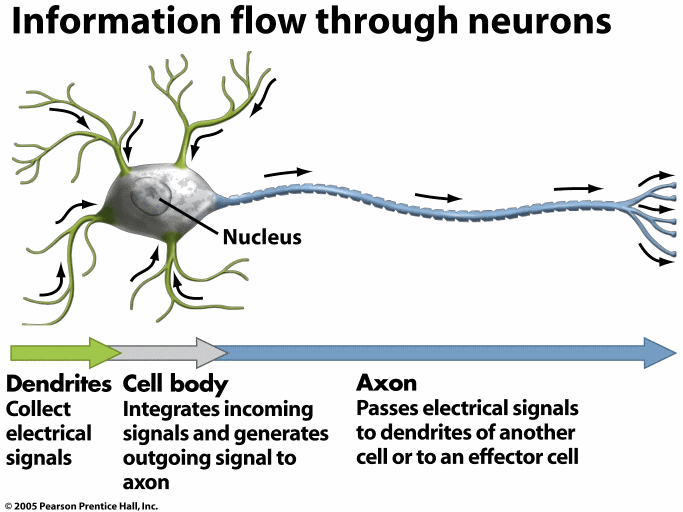
\includegraphics[width=0.43\textwidth]{neuron}
  \end{center}
  \caption{Inside a cell wall.}
  \label{fig:neuron}
  \vspace{-5pt}
\end{wrapfigure}
The structure of the axon is shown schematically in figure~\ref{fig:axMod1} below.
For electrical purposes, an axon is basically a long, thin cylinder of membrane filled with a fluid called axoplasm.
When no action potential is traveling, the potential difference across the membrane, from the outside of the axon to the inside, is about -70 mV, the resting potential difference.
In part, this is because the concentration of of sodium atoms (Na$^{+}$) is much higher outside the axon than inside.
\par
The axoplasm, like all fluids in biological systems, has mobile ions dissolved in it, giving it a moderate conductivity (many orders of magnitude lower than copper or other metals we can think of as ideal conductors).
the fluid outside the membrane, the extra-cellular fluid, is very similar to the axoplasm and thus has approximately the same conductivity.
\par 
The lipid bilayer forming the membrane is electrically insulating, with extremely low conductivity, but many different kinds of channel proteins cross the membrane.
These channels only allow specific ions to pass under particular conditions,
the channels increase the conductivity of the membrane as a whole, so that although the membrane conductivity is much lower than that of the axoplasm, current does not pass through the membrane.
\begin{figure}[hbtp]
	\centering
	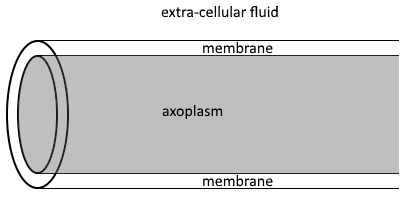
\includegraphics[width=0.4\textwidth]{axonModel1}
	\caption{Simple cylinder model of an axon.}
	\label{fig:axMod1}
\end{figure}

\section*{Part 1: Modeling Passive Transport}
Our goal is to understand how a potential difference applied across the membrane at one end of the axon spreads along the axon if it is not being regenerated as it travels down the axon.
thus for the purposes of our model we'll assume there is a battery at the left end of the axon segment (see figure~\ref{fig:axMod2}), holding the potential difference from the outside to the inside at $x=0$ to a positive value we'll call $V_{0}$.
\begin{wrapfigure}{R}{0.45\textwidth}
  \vspace{-25pt}  
  \begin{center}
    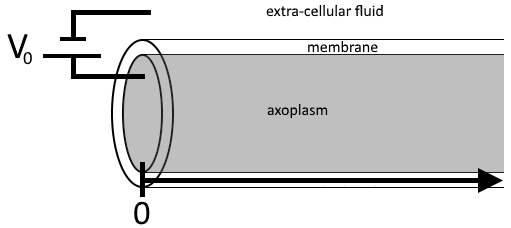
\includegraphics[width=0.43\textwidth]{axonModel2}
  \end{center}
  \caption{Model of potential difference across axon membrane.}
  \label{fig:axMod2}
  \vspace{-5pt}
\end{wrapfigure}
\par 
Suppose there was just a single ion channel (e.g., a `potassium leak channel') crossing through the membrane, at the right end of the segemnt in the figure. 
Draw a loop onto the diagram showing the path of current flow from the positive side of the battery (inside) to the negative side of the battery (outside), and then draw a simple circuit that corresponds to this pattern of current flow.
The axoplasm, an ion channel, and the extra-cellular fluid should each be represented separately in your simple circuit.
\par 
In fact, the resistance of the current path through the extra-cellular is much less than the resistance of either the axoplasm or the ion channel through the membrane, so the extra-cellular fluid can be represented as just a conducting wire in the simple circuit.
(If you didn't initially do so, update your simple circuit accordingly.) 
Let's think about why the extracellular fluid will have such low resistance.
\par 
Resistance $R$ can be determined from the length $L$, the cross-sectional area $A$, and the resistivity $\rho$ according to $R = \frac{\rho L}{A}$.
The resistivities of the axoplasm and the extracellular fluid are very similar.
Considering how the current flows through both the axoplasm and the extra-cellular fluid, explain why the resistance of the current path through the extra-cellular fluid is much smaller than the resistance of the current path through the exoplasm - thus we cannot treat the extra-cellular fluid as just a conducting wire.
\par 
A long axon can be modeled as a chain of many short segments like the segments like the segment described above.
The dashed lines in figure~\ref{fig:axMod3} visually divide the axon into five such segments.
sketch the path of current flow onto the diagram and then design a circuit model for it.
Check your model with your instructor.
\par 
\begin{wrapfigure}{R}{0.45\textwidth}
  \vspace{-15pt}  
  \begin{center}
    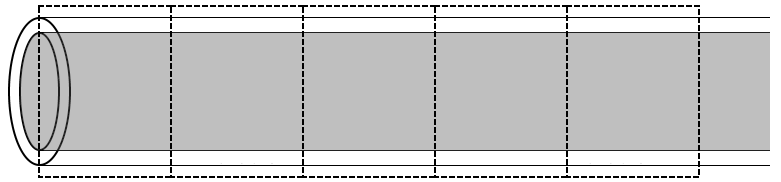
\includegraphics[width=0.43\textwidth]{axonModel3}
  \end{center}
  \caption{Axon chain of many segments.}
  \label{fig:axMod3}
  \vspace{-5pt}
\end{wrapfigure}
To complete the model, we need values for the resistances.
There are actually many ion channels passing through the membrane, so our circuit model needs to be constructed using the resistance of a segment of membrane rather  than a single ion channel.
Each segment of membrane consists of many ion channels in parallel, so the overall resistance of the membrane segment is the equivalent resistance of all of those ion channels. 
The average resistivity of the membrane can be measured and used to find the resistance of a segment of membrane.
\par 
Use the relationship between resistance, resistivity, length, and cross-sectional area to estimate values for the resistance of a membrane segment $R_{mem}$ and an axoplasm segment $R_{axon}$ using the following order-of-magnitude values:
\begin{itemize}
\itemsep-0.2em
\item the diameter of the axon $\sim$ 10 $\mu$m
\item the membrane thickness $\sim$ 10 nm
\item the resistivity of the axoplasm $\sim$ 1 $\Omega$-m
\item the average resistivity of the membrane $\sim  10^{8} \; \Omega$-m
\item the segment length $\sim$ 1 mm
\end{itemize}
Hint: To determine the cross-sectional area of a membrane segment, think of unrolling the membrane from the axon.
Also, it turns out that only the ratio $R_{mem}/R_{axon}$ affects how far the potential difference will spread.

\section*{Part 2: Qualitative Analysis of Your Model}
With the model you have created, we hope to understand how the potential difference across the membrane changes as we examine different distance along the nerve axon.
In other words, how is the voltage across the membrane at a distance $x$ related to the initial voltage $V_{0}$?
Before we collect data and perform a quantitative analysis of your model, let us think qualitatively about some of the features of your model of passive transport.
\par 
We want to understand how the voltage across the membrane depends on the distance along the axon.
Each segment in you multi-segment model circuit should include a resistor representing the membrane, so the voltages across these resistors represents $V_{mem}$ at eachsegment.
The first $R_{mem}$ corresponds to segment 1, the second to segment 2, and so on. 
Let's notate these voltages as $V_{mem}^{1}$, $V_{mem}^{2}$, and so on.
Similarly, let's call the voltages across the axon segments $V_{axon}^{1}$, $V_{axon}^{2}$, and so on; the currents in the axon segments are $I_{axon}^{1}$, $I_{axon}^{2}$, and so on.
\par 
\textbf{Applying the loop rule} to the first segment, find in terms of the applied membrane potential $V_{0}$, the current in the first axon segment $I_{axon}^{1}$, and the membrane resistance $R_{axon}$.
Do the same for the second segment, finding $V_{mem}^{2}$ in terms of the applied membrane potential $V_{0}$, the axon currents, and the resistance $R_{axon}$.
\emph{Is $V_{mem}^{2}$ less than, equal to, or greater than $V_{mem}^{1}$? How do you know?}
Do the same for the third segment, finding $V_{mem}^{3}$ in terms of the applied membrane potential, the currents in the segment, and the axon resistance.
With $n$ indicating the segment number, does $V_{mem}^{n}$ increase or decrease as $n$ increases?
Does $I_{axon}^{n}$ increase or decrease as $n$ increases? 
On your circuit diagram, draw arrows of different widths (or lengths) by each axon resistor to indicate the amount of current in the axon segment.
\par 
From your analysis, it should be clear that $V_{mem}$ decreases as you go further and further from the start of the axon.
Can we be more specific?
If we create a mathematical model for $V_{mem}(x)$ as a function of $x$, where x is the distance from the start of the axon, what functional form would we expect?
As a reminder, common possibilities include:
\begin{enumerate}
\itemsep-0.2em
\item linear with a negative slope (rate of change is constant)
\item inverse (product is constant)
\item exponential decay (percent change is constant)
\end{enumerate}
It should help to consider the behavior of $V_{mem}(x)$ in the limiting cases.
Examine the behavior of your model circuit.
As $x$ approaches $0$, what happens to $V_{mem}(x)$?
As $x$ becomes very large, what happens to $V_{mem}(x)$?
Compare with the behavior of each of the possible functional forms.
Make your best guess for the functional form and sketch the corresponding graph of $V_{mem}(x)$ vs. $x$.
Explain your reasoning.

\section*{Part 3: Quantitative Analysis of Your Model}
We are now ready to build and test your passive transport circuit model.
\par 
Equipment:
\begin{itemize}
	\itemsep-0.2em
	\item circuit board
	\item connecting wires
	\item alligator clips
	\item battery 
	\item switch
	\item assorted resistors (10 each of three different kinds)
	\item voltage probe
	\item LabPro
	\item computer and LoggerPro software
\end{itemize}
The circuit board (also known as a ``breadboard'') is probably new to you and requires a short explanation (see figure~\ref{fig:breadboard}).
Down the edges of the board are two columns of holes surrounded by a red and a blue line.
Leave the negative end of the battery connected to the blue line; this is your extra-cellular fluid and all of these holes are connected together in this column (connected inside the circuit board).
The other parts of the circuit board are much wider sets of columns.
For these, the holes in a column are NOT connected, but the holes in a row ARE connected.
If this is not clear enough for you, please ask your TA to explain.
You will need to think carefully about how you can fit your model of passive transport in a nerve axon onto this circuit board.
You have two circuit boards so that you can begin building a second model with spare resistors once you are ready to test the first model.
\par 

\begin{figure}[hbtp]
	\centering
	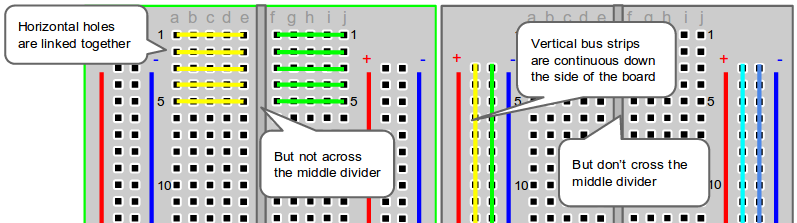
\includegraphics[width=\linewidth]{breadboard-connect.png}
	\caption{Breadboard connections diagram.}
	\label{fig:breadboard}
\end{figure}

\textbf{Construct your model circuit with ten segments} using the provided components.
Choose resistors with the proper ratio of resistance values that you found in the previous part, and make sure that you use the same value value of resistance for all of the $R_{mem}$ and a different constant value for all of the $R_{axon}$.
Don't forget to close the switch to take data and open it when you finish.
\par 
\textbf{Measure and record} $V_{mem}$ vs. $x$ for $x = 0 \, mm$ to $x = 10 \, mm$.
(In your circuit, each axon resistor corresponds to a 1 mm segment, so for your measurements, x is the segment number.
At $x=0$, $V_{mem}(x)=V_{0}$.)
To record voltages in LoggerPro:
\begin{itemize}
\itemsep-0.2em
\item Click on the Data Collection icon, and change the mode to ``Events with Entry.'' Provide appropriate name and units. Click `Done'.
\item Press the start button.
\item Use the voltage probe to measure voltages by attaching the probe leads to the circuit on either side of each $R_{mem}$. To store voltage values in a table, click on `Keep Current Value'. You can enter the corresponding length value in the same row of the table. Don't forget to collect the $x=0$ value $V_{0}$!
\item If a Data Erase box appears, click on `Append to Latest Data' and proceed.
\item Press the stop button when finished with all 11 data points.
\item To display data points without connecting lines, double click on the graphed data, and unselect the option for connecting the data points.
\end{itemize}
Now let's \textbf{interpret your results}.
Following the same line of reasoning you used in your qualitative analysis to find $V_{mem}^{n}$, and assuming that the segment is only a different length $dx$ long, it is possible to derive a differential equation for $V_{mem}(x)$ - don't do this, just know that it is possible!
Solving the differential equation gives us an equation describing how the voltage across the membrane depends on the distance $x$ from the end where a voltage $V_{0}$ is applied.
The equation is then:
\[ V_{mem}(x) = V_{0} e^{-x/\lambda} \quad \textrm{with} \quad \lambda =\alpha \sqrt{\frac{R_{mem}}{R_{axon}}}  \]
where $\lambda$ (Greek letter lambda, called the length constant of the axon) is the distance along the axon at which $V_{mem}(x)$ has decreased by a factor of $e$ (the natural logarithm base e), to $0.37 V_{0}$, and $\alpha$ is a proportionality constant with units of length that is specific to different types of axons.
\par 
To perform a fit:
\begin{itemize}
\itemsep-0.2em
\item Click `Analyze'.
\item From the drop-down menu select `curve fit'.
\item From the pop-up menu select the appropriate function for exponential decay.
\item Click `Try Fit'.
\item If it is the correct fit click `Ok'.
\end{itemize}
Provide the graph of your data with your best fit function in your lab write-up.
Calculate the length constant of your model circuit from your best fit function.
What does this length constant tell you about the feasibility of passive transport as a signal transmission method?
Will your brain ever be informed of an injury to your toe?
Given the length constant you have determined, how many `lengths' are there in the nerve connecting your toe to the base of your spine?
What fraction of the original potential difference ($V_{0}$ at your toe) remains by the time the signal reaches the spine?
\par 
Build two new model circuits with two different length constants and find these length constants with a few measurements (you don't have to measure as many data points if you choose them wisely; include the graphs for these two circuits in your report).
(\textbf{\emph{Hint:}} You have three different sets of resistors. 
How many ways can you pair them up to build a circuit? 
What ways have you already used?)
How does the length constant change as the ratio of $R_{mem}$ to $R_{axon}$ changes?
To get a signal from your toe to reach the base of your spine using passive transport, \textbf{what would the ratio of the resistance need to be}?
State your assumptions.

\newpage

\section*{Part 4: What adaptations allows the action potential to travel faster?}
How fast does an action potential travel along an axon?
You're probably aware that it's finite - no one has truly instant reflexes.
Yet, your model circuit suggests that the process is nearly instantaneous.
Something is missing from the model.
We need to extend our model in order to understand \emph{why} it takes time for an action potential to travel along an axon.
\par 
Let's take a closer look at the membrane of an axon.
[See figure 5 below.]
The channels are the paths through which ions flow (with some resistance).
The equivalent resistance of all of these parallel channels in a single segment is $R_{mem}$.
Now take away those channels and what do you have left?
An insulating layer with conducting fluids on each side.
That should remind you of a familiar device - a capacitor.
The membrane is therefore properly viewed as a resistor and a capacitor in parallel.
[See figure 6 below.]
As current travels along the axon and enters each new segment, charge also accumulates on the capacitor.
It takes a significant amount of time for a capacitor to charge and thus also for the potential difference across the membrane to reach its final destination.
We refer to the time it takes the membrane potential difference to reach 63\% of its final value as the time constant $\tau$.
It can be shown that $\tau = R_{mem}C_{mem}$, where $R_{mem}$ is the resistance and $C_{mem}$ is the capacitance of a segment of membrane.
It takes several time constants for the membrane potential difference to reach the values that your model resistor circuit gives.
\begin{figure}[hbtp]
\centering
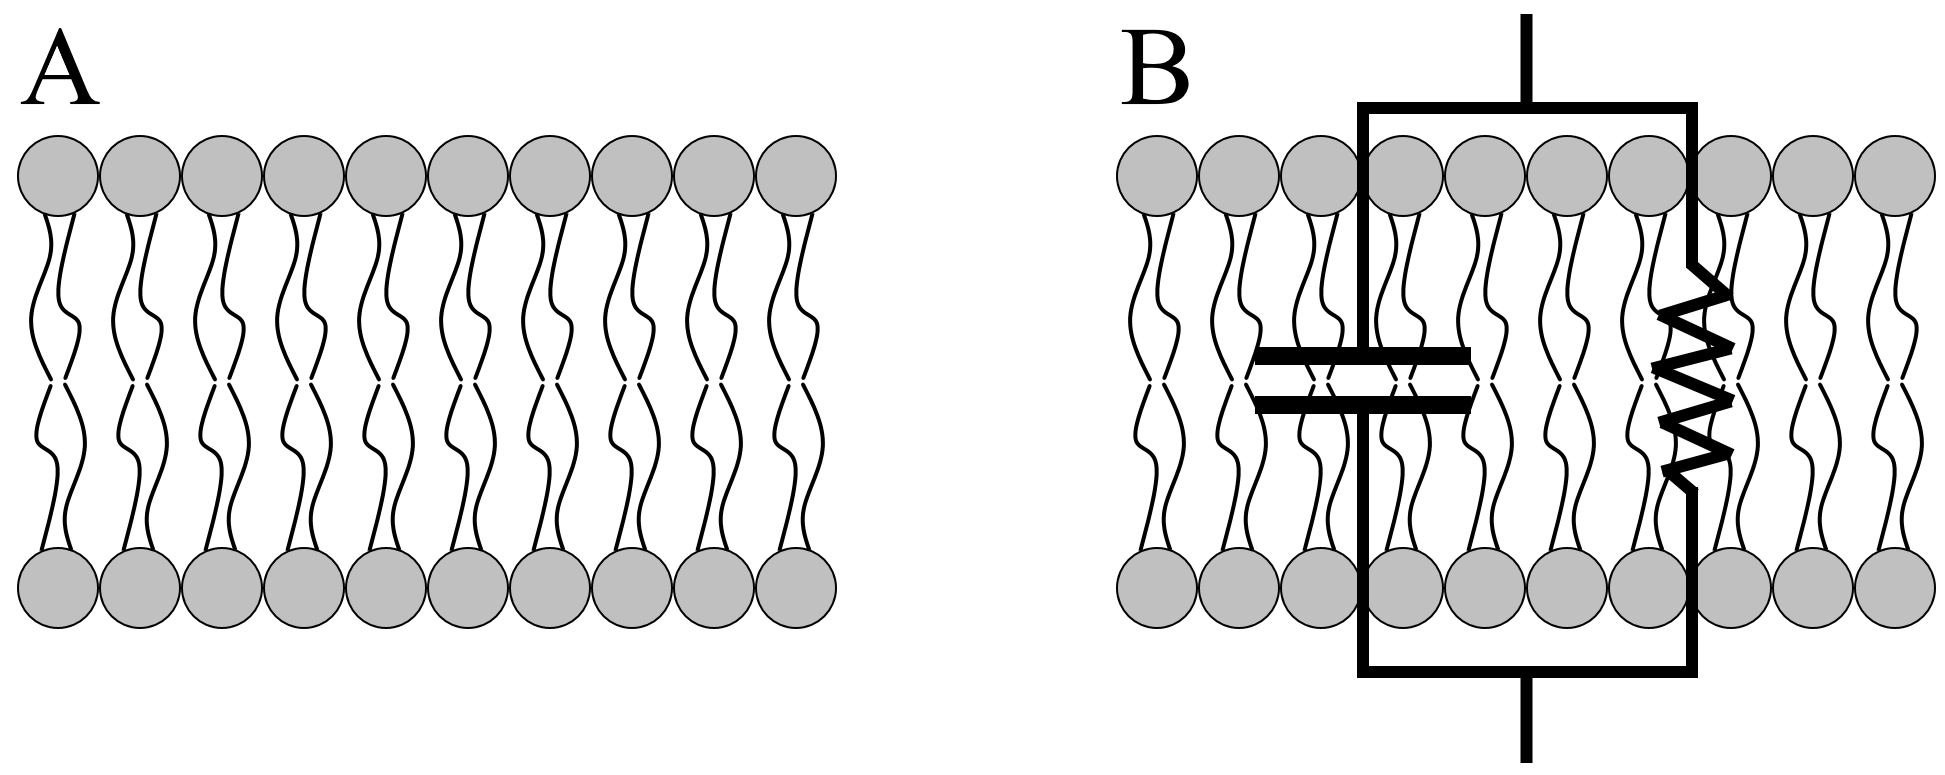
\includegraphics[width=0.5\textwidth]{membraneRC}
\caption{(A) magnified view of a membrane. (B) RC circuit model of a membrane.}
\label{fig:memRC}
\end{figure}


\subsection*{Speed depends on time constant and length constant}
The speed at which an action potential travels down an axon depends primarily on two things:
\begin{itemize}
\itemsep-0.2em
\item \textbf{It's \emph{inversely proportional} to the time constant:} The longer it takes the membrane potential difference to rise in each segment, the slower the action potential will travel. The time constant is given by $\tau = R_{mem}C_{mem}$.
\item \textbf{It's \emph{proportional} to the length constant:} The greater the length constant, the farther the depolarizing potential difference reaches down the axon without regeneration, bringing successive segments to the threshold potential difference required to regenerate the action potential sooner. You measured the length constant of your model circuit in Part 3. In general, the length constant $\lambda$ is proportional to $\sqrt{R_{mem}/R_{axon}}$. This makes sense: If the membrane resistance is really big (or if the axon resistance is really small), current mostly flows \emph{down} the axon, with just a little flowing across the membrane in each successive segment.
\end{itemize}
It makes sense that faster propagation of nerve impulses confers an advantage to an organism.
In the next few questions, we'll \textbf{examine the physics behind some adaptations leading to speedier action potentials}.

\begin{figure}[hbtp]
	\centering
	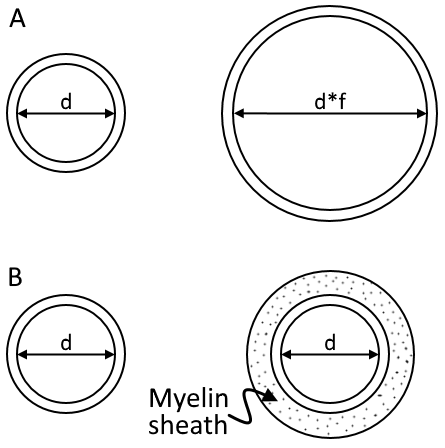
\includegraphics[width=0.5\linewidth]{axon_alt}
	\caption{caption}
	\label{fig:axon_alt}
	\vspace{-20pt}
\end{figure}

\subsection*{How does making the axon wider affect the speed?}
Let's say the diameter of the axon is increased by a factor of $f$. [Figure~\ref{fig:axon_alt}A]
\begin{enumerate}
\itemsep-0.2em
\item By what factor does $R_{axon}$ change? (Note: The resistivity of the axoplasm is constant, as is the 1 mm length of an axon segment.)
\item By what factor does $R_{mem}$ change? (Note: The resistivity of the membrane is constant, as is the 1 nm thickness of the membrane.)
\item By what factor does the length constant $\lambda$ change?
\item Assuming that the time constant doesn't change, by what factor does the speed therefore change?
\item By what factor would the diameter of the axon have to change to increase the speed by a factor of 10?
\end{enumerate}
Note: The `wider axon adaptation' is the strategy adopted by the squid, whose `giant' axons allow very rapid travel of its action potentials, making it a master of the quick escape.

\newpage

\subsection*{What about making the membrane thicker?}
Wider axons work fine for a squid, but are highly impractical for organisms with lots of neurons like humans.
(If each of your neurons were the size of a squid's, your head wouldn't fit through a doorway!)
Let's explore another possible way of increasing the length constant and therefore the speed: increasing $R_{mem}$.
This is a strategy commonly adopted by vertebrates.
It's achieved by extra insulation (a myelin sheath) that's wrapped around the axon. [Figure~\ref{fig:axon_alt}B]
\begin{enumerate}
\itemsep-0.2em
\item Let's say that myelination increases the membrane resistance by a factor of 1000. By what factor does the length constant increase? Why?
\item Assuming that the time constant doesn't change, by what factor do the speed therefore change? Why?
\item Based on the analysis you did in part 3, could a myelinated axon use passive transport as the signal transmission method? Why or why not?
\item There are many diseases that affect signal transmission along neural pathways. These include multiple sclerosis (MS), myasthenia gravis, and amyotrophic lateral sclerosis (ALS or `Lou Gehrig's Disease'). Often, a component of these afflictions is a malformation or degeneration of the myelin sheath. MS is a demyelinating disease, which means that the axons of neurons are intact but the myelin sheaths are damaged. Why would loss or damage to the myelin sheath be a problem for signal transmission, even if the axon was intact?
\end{enumerate}
Note: Myelination obstructs the membrane's voltage-gated Na$^{+}$ channels that enable the action potential to be regenerated.
For this reason, there are gaps in the myelin coating, called the nodes of Ranvier, where the channels are not obstructed.
From what you've learned in this lab, what do you suppose determines the maximum distance between these gaps?

\section*{For your report:}
As stated previously, the \textbf{lab write-up} should include (a) your explanations of the models you made, (b) the supported conclusions you drew from analyses of your models, and (c) your discussion of advanced topics related to the basic ideas yoiu are exploring.
To be more specific, you should discuss the work you have done and the considerations you have made in modeling passive transport, qualitatively and quantitatively analyzing your model, and modeling adaptations that can increase the speed of signal transfer.
If you want to include hand-drawn elements (such as model circuit diagrams), please do so.
Don't forget to include the plots of $V_{mem}(x)$ vs. $x$ with the appropriate fitting functions. 
\underline{Respond explicitly} to all passages marked with an exclamation point (!).
